%%%-------------------------------------------------%%%
%%% Sub document results %%%
%%%-------------------------------------------------%%%

\section{Results}

% Remove the lipsum and the example plots and tables to fill in your abstract text here

\subsection{Subheading}

\lipsum[1-2]

\begin{figure}[H] % {{{
   \centering
      \begin{tikzpicture}
	 \node[pictureframe]{%    
	    \begin{minipage}{0.47\textwidth}%
	       \begin{center}
\begin{knitrout}
\definecolor{shadecolor}{rgb}{0.969, 0.969, 0.969}\color{fgcolor}
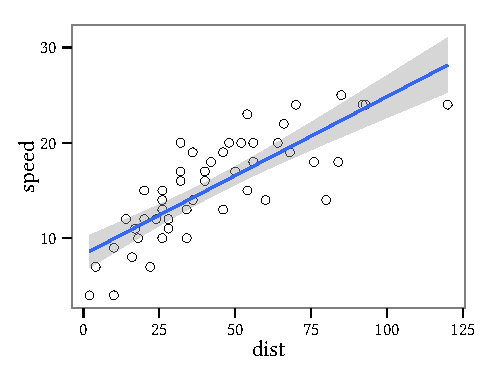
\includegraphics[width=\maxwidth]{usr/graphics/dynamic/test_plot} 

\end{knitrout}

	       \end{center}
	    \end{minipage}
	 };
      \end{tikzpicture}
   \caption{Lorem ipsum dolor sit amet, consectetuer adipiscing elit. Aenean
   commodo ligula eget dolor. Aenean massa. Cum sociis natoque penatibus et magnis
   dis parturient montes, nascetur ridiculus mus. Donec quam felis, ultricies nec,
   pellentesque eu, pretium quis, sem.}
\label{fig:test_plot}
\end{figure} % }}}

\lipsum 

\begin{equation}
   \sqrt[3]{1-y^2}
\end{equation}

\setlength\multlinegap{0pt}
\begin{multline} \tag{2}
   \sum_{t \in \mathbf{T}} \int_a^t
   \biggl\lbrace \int_a^t f(t - x)^2 \,
   g(y)^2 \,dx \biggr\rbrace \,dy \\
   = \sum_{t \notin \mathbf{T}} \int_t^a
   \biggl\lbrace g(y)^2 \int_t^a
   f(x)^2 \,dx \biggr\rbrace \,dy
\end{multline}

\begin{figure*} % {{{
   \centering
      \begin{tikzpicture}
	 \node[pictureframe]{%    
	    \begin{minipage}{0.98\textwidth}%
	       \begin{center}
\begin{knitrout}
\definecolor{shadecolor}{rgb}{0.969, 0.969, 0.969}\color{fgcolor}
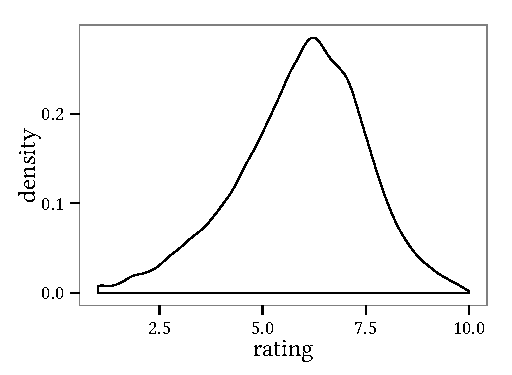
\includegraphics[width=\maxwidth]{usr/graphics/dynamic/test_plot_two1} 
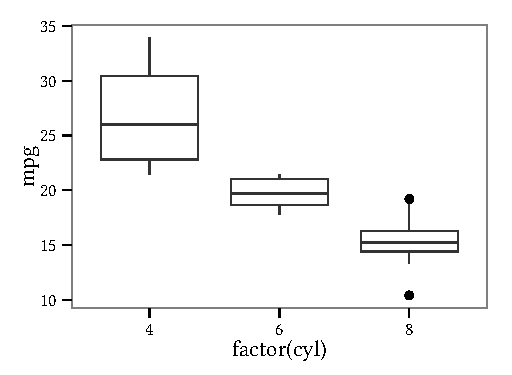
\includegraphics[width=\maxwidth]{usr/graphics/dynamic/test_plot_two2} 

\end{knitrout}

	       \end{center}
	    \end{minipage}
	 };
      \end{tikzpicture}
   \caption{Lorem ipsum dolor sit amet, consectetuer adipiscing elit. Aenean
   commodo ligula eget dolor. Aenean massa. Cum sociis natoque penatibus et magnis
   dis parturient montes, nascetur ridiculus mus. Donec quam felis, ultricies nec,
   pellentesque eu, pretium quis, sem.}
\label{fig:test_plot_two}
\end{figure*} % }}}

\lipsum[1-4]

\begin{lstlisting}[language=Ruby]
#!/usr/bin/ruby

$i = 0
$num = 5

while $i < $num  do
   puts("Text inside the loop: i = #$i")
   $i +=1
end
\end{lstlisting}

% example for a two column table %

\begin{table*} % {{{
% Label tab:test_plot_two 
	\centering
	\label{tab:test_table_two}
	\caption{Lorem ipsum dolor sit amet, consectetuer adipiscing elit. Aenean
	 commodo ligula eget dolor. Aenean massa. Cum sociis natoque penatibus et magnis
	 dis parturient montes, nascetur ridiculus mus. Donec quam felis, ultricies nec,
	 pellentesque eu, pretium quis, sem.}
	   {\small
		\begin{tabular}{p{0.08\textwidth}p{0.08\textwidth}p{0.08\textwidth}p{0.08\textwidth}p{0.08\textwidth}p{0.08\textwidth}p{0.08\textwidth}p{0.08\textwidth}p{0.08\textwidth}}
				\toprule
				   \multicolumn{4}{c}{A-D}   & \multicolumn{5}{c}{E-I}\\
				\cmidrule(lr){1-4} \cmidrule(lr){5-9}
					A     & B & C & D & E & F & G & H & I\\
				\midrule
					1     & 2 & 3 & 4 & 5 & 6 & 7 & 8 & 9\\
					1     & 2 & 3 & 4 & 5 & 6 & 7 & 8 & 9\\
					1     & 2 & 3 & 4 & 5 & 6 & 7 & 8 & 9\\
					1     & 2 & 3 & 4 & 5 & 6 & 7 & 8 & 9\\
				\bottomrule
			\end{tabular}
		}
\end{table*} % }}}



